\head{Февраль}{Листок 5. Теория множеств.}
\epigraph{\textit{Множество есть многое,} \\ \textit{мыслимое нами как единое.}}{Георг Кантор}\epigraph{\textit{- Они рисовали мышеловки, месяц, математику, множество... 
Ты когда-нибудь видела, как рисуют множество? - спросила Соня.}
\\
\textit{- Множество чего? - спросила Алиса.}
\\
\textit{- Ничего, - отвечала Соня. - Просто множество!}}{Льюис Кэрролл, "Алиса в стране чудес."}

Что такое \textit{множество}? Наверно, каждый математик хоть раз задумывался, что это такое. В обычной жизни каждый из нас легко использует это понятие. Это некий набор предметов, утверждений, каких-либо
объектов. Будь это множество целых чисел, корней уравнения, геометрическое множество точек на плоскости, множество спутников Юпитера, всех Александров на Земле, арифметических операций или даже хрюкающих фрюкозябриков. Объекты, составляющие множество, называются его \textit{элементами}.\footnote{Считают, что один и тот же элемент не может входить в множество дважды. Таким образом, множество {2, 2, 3} есть
не что иное, как множество {2, 3}, просто представленное другой записью.} В жизни, употребляя слово "множество", подразумевается, что тех "элементов", о которых идёт речь, - "много". Совсем другое дело в математике - множество может состоять из одного, двух элементов, или даже не содержать ни одного элемента. Такое множество без элемента, называется пустым множеством и обозначается знаком $\varnothing$. Таковым, например, является множество всех летающих крокодилов.

{\setlength{\intextsep}{2pt}
\begin{figure}[h]
\begin{minipage}[h]{0.8\linewidth}\setlength{\parindent}{1.5em}
    \begin{ex}\label{5.0 u1}Что представляют собой следующие множества:
    \par
    а)~множество натуральных делителей числа 12;
    \par
    б)~множество точек, равноудалённых от двух данных;
    \par
    в)~множество точек, равноудалённых от трёх данных, не лежащих на прямой;
    \par
    г)~множество точек, равноудалённых от трёх данных, лежащих на прямой;
    \par
    д)~множество точек, равноудалённых от двух пересекающихся прямых;
    \par
    е)~множество букв, используемых при написании слова СПЕЦМАТЕМАТИКА?
    \end{ex}
\end{minipage}
\hfill
\begin{minipage}[h]{0.19\linewidth}
    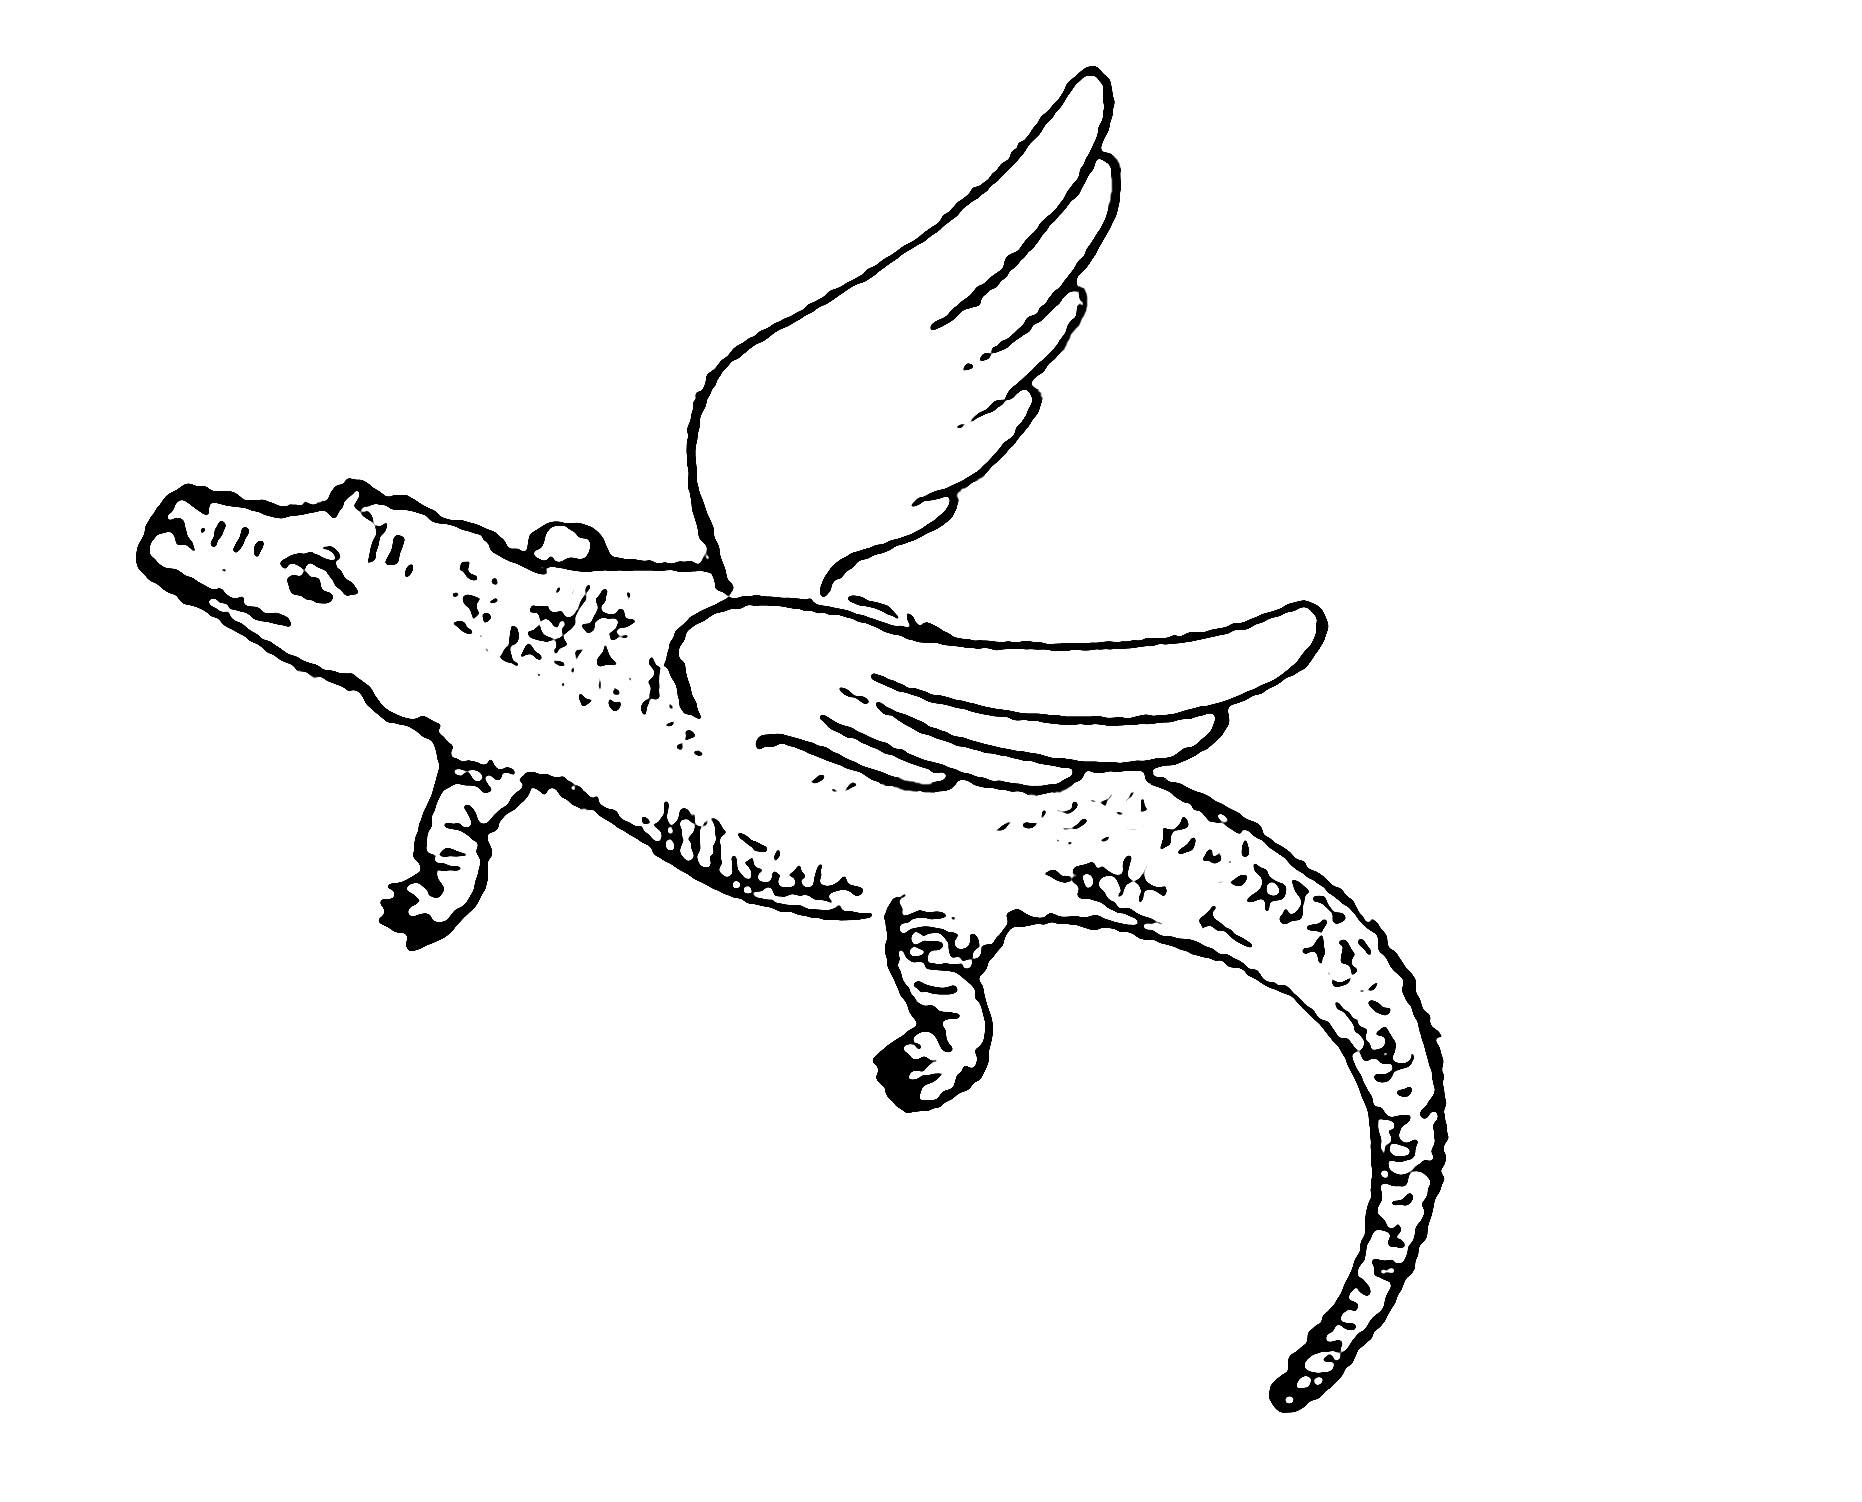
\includegraphics[width=0.9\columnwidth]{./img/krokodil}
\end{minipage}
\end{figure}}

Дадим ещё несколько определений:
\begin{dfn}
Множество $X$ называется \textit{подмножеством} множества $Y$, если каждый элемент множества $X$ принадлежит множеству $Y$. Обозначение: $X \subset Y$. Пустое множество является подмножеством любого множества.
\end{dfn}

\begin{ex}\label{5.0 u2}
Докажите, что множество $X$ является подмножеством множества $Y$ тогда и только тогда, когда любой элемент, не принадлежащий $Y$, не принадлежит и множеству $X$.
\end{ex}

\begin{dfn}
Множества $X$ и $Y$ \textit{равны}, если $X \subset Y$ и $Y \subset X$, т.е. если они состоят из одних и тех же элементов.
\end{dfn}

\begin{dfn}
\textit{Пересечением} множеств $A$ и $B$ называется множество $A \cap B = \{x~|~x \in A~\textit{и}~x \in B\}$. В частности пересечением бесконечного семейства множеств называется множество, состоящее из тех и только тех элементов, которые принадлежат каждому множеству этого семейства.
\end{dfn}

\begin{dfn}
\textit{Объединением} множеств $A$ и $B$ называется множество $A \cap B$ = $\{x~|~x \in A~\textit{или}~x \in B\}$. В частности объединением бесконечного семейства множеств называется множество, состоящее из тех и только тех элементов, которые принадлежат хотя бы одному множеству этого семейства.
\end{dfn}

\begin{dfn}
\textit{Разностью} множеств $A$ и $B$ называется множество $A \setminus B = \{x~|~x \in A~\textit{или}~x \notin B\}$.
\textit{Симметрической разностью} множеств $A$ и $B$ называется множество $A \Delta B = \{x~|~x \in A \setminus B~\textit{или}~x \in B \setminus A\}$.
\end{dfn}

{\setlength{\intextsep}{2pt}
\begin{figure}[H]
\begin{minipage}{0.74\linewidth}\setlength{\parindent}{1.5em}
\begin{ex}\label{5.0 u3}
    Выразите пересечение $A \cap B$, используя только операции разности множеств.
\end{ex}
   \begin{ex}\label{5.0 u4}На рисунке изображены три множества: $A$, $B$ и $C$. Изобразите следующие множества:
    а)~$(A \cap B)\cup C$;
    ~
    б)~$(A \cup B)\cap C$; 
    \par
    в)~$(A \setminus B)\cap C$;
    ~
    г)~$(C \setminus B)\cap(C \setminus A)$;
    ~
    д)~$(A \Delta B)\cap(A \Delta C)$
    \end{ex}
    \begin{thm}
Докажите, что для любых множеств $A$, $B$ и $C$ справедливо соотношение $(A \cup B) \cap C = (A \cap C) \cup (B \cap C)$
\end{thm}
\end{minipage}
\hfill
\begin{minipage}{0.25\linewidth}
    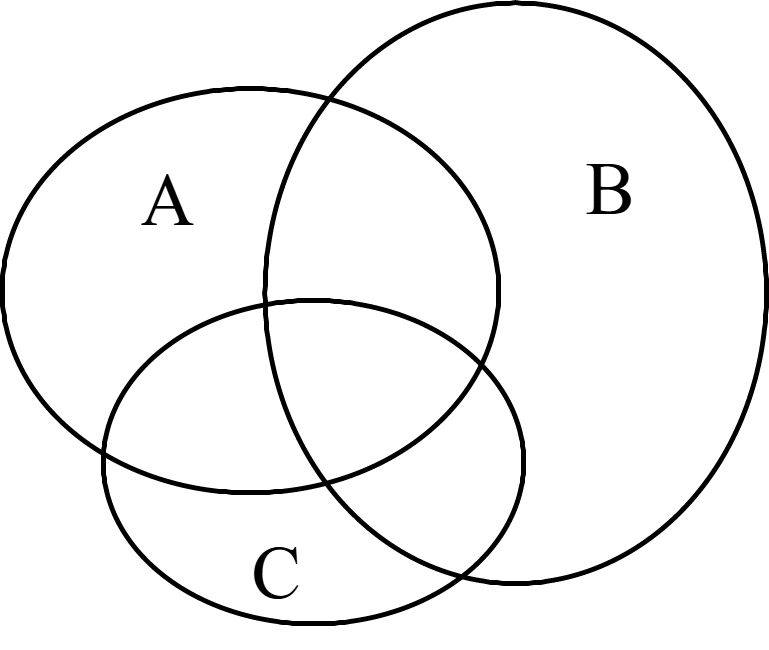
\includegraphics[width=0.9\columnwidth]{img/euler.png}
\end{minipage}
\end{figure}}

\begin{prf}
Если мы докажем, что все элементы множества из левой части принадлежат множеству из правой части требуемого равенства и наоборот, что все элементы множества из правой части принадлежат множеству из левой части, то утверждение будет доказано. Пусть элемент $x \in (A \cup B) \cap C$. Это значит, что $x$ принадлежит одновременно множеству $C$ и объединению множеств $A$ и $B$.\footnote{Объединение множеств $A$ и $B$ можно разбить на три части (некоторые из них, возможно, пустые): элементы, принадлежащие
только $A$, элементы, принадлежащие только $B$ и элементы, принадлежащие одновременно и $A$, и $B$ (т.е. пересечению $A$ и $B$).} Если $x \in (A \cup B)$, то это значит, что он обязательно принадлежит или $A$, или $B$. Следовательно, если $x \in A$, то он принадлежит пересечению множеств $A$ и $C$ и, значит, принадлежит множеству, из правой части. Аналогично, если $x \in B$. Таким образом, если $x \in (A \cup B) \cap C$, то $x \in (A \cap C) \cup (B \cap C)$. Докажем теперь, что если $x \in (A \cap C) \cup (B \cap C)$, то $x \in (A \cup B) \cap C$. Пусть $x$ принадлежит объединению пересечений множеств $A~и~C$ и $B~и~C$. Следовательно, он принадлежит $C$ и одному из множеств $A$ или $B$ (а может быть обоим сразу). Условие того, что элемент принадлежит или множеству $A$, или множеству $B$ означает, что $x \in (A \cup B)$. Значит, $x \in (A \cup B) \cap C$.
\end{prf}

\begin{ex}\label{5.0 u5}
Составьте всевозможные пересечения и объединения следующих множеств:
\par
$A = \{1; 2; 3; 4; 5; 6; 7; 8; 9\}$
$B = \{8; 3; 5; 10 ;4\}$ $C = \{6; 7; 9; 4; 8; 10; 11; 12\}$  $D=\{10; 9; 8\}$.
\end{ex}

{\setlength{\intextsep}{2pt}
\begin{figure}[H]
\begin{minipage}{0.19\linewidth}
    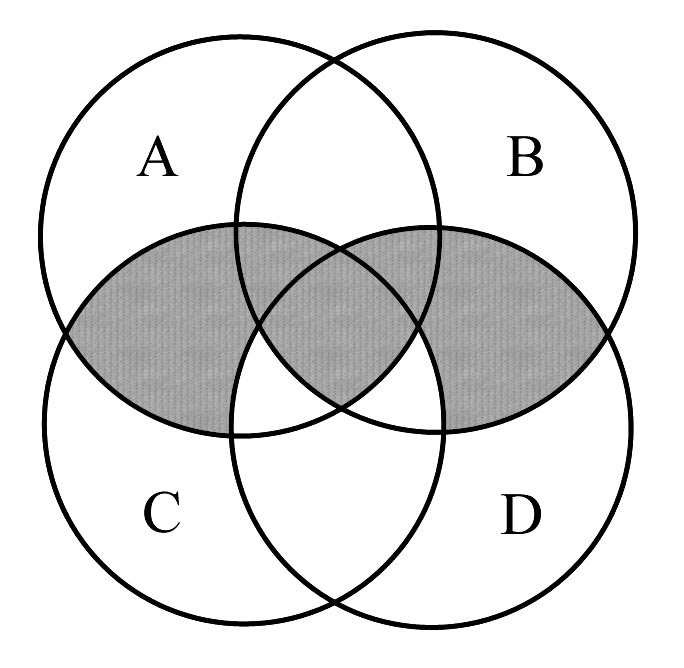
\includegraphics[width=0.9\columnwidth]{./img/euler2}
\end{minipage}
\hfill
\begin{minipage}{0.8\linewidth}\setlength{\parindent}{1.5em}
\begin{thm}
Найдите подмножества $X$ и $Y$ множества $A$, состоящего из 25 сердитых индюков, если для любого подмножества $B \subset A$ выполнено равенство $X \cap B = Y \cup B$. А если множество $A$ любое и даже не индюков? \textit{(Обсудите эту задачу в классе)}
\end{thm}

    \begin{thm}
    Даны четыре множества $A$, $B$, $C$ и $D$, изображённые на рисунке слева. При помощи операций $\cap$, $\cup$, $ \backslash $ и $\Delta$ выразите закрашенное множество $M$ через $A$, $B$, $C$ и $D$.
    \end{thm}
\end{minipage}
\end{figure}}

\section{Метод кругов Эйлера}
\epigraph{
\textit{"В будущем все комнаты в домах будут круглые"}
\par
\textit{"Это почему ещё?"}
\par
\textit{"А чтобы родители не могли ставить детей в угол!}}{Из разговора в песочнице.}

Некоторые задачи очень легко решаются, если их переформулировать на язык множеств. Удобно изображать множества в виде кругов (или диаграмм) на плоскости, которые делят её на куски. Например, для множеств $A$ и $B$ получим четыре куска (множества): $\{x~|~x \in A~и~x \in B\}, \{x~|~x \in A~и~x \notin B\}, \{x~|~x \notin A~и~x \in B\}, \{x~|~x \notin A~и~x \notin B\}$.

Такой метод схемы получил название метода кругов (или диаграмм) Эйлера.\footnote{Иногда такие диаграммы называют также диаграммами Эйлера – Венна}

\begin{ques}
    На сколько частей разделят плоскость "круги Эйлера" для 3 множеств? 
    \par
    А 5?
\end{ques}

\begin{thm} (задача - шутка) Кого больше: котов, кроме тех котов, которые не являются Васьками, или Васек, кроме тех Васек, которые не являются котами? \hfill :-)
\end{thm}
\begin{thm}
Петя и Вася разучивали песни. Оказалось, что из сборника "Наши любимые песни" Петя знает 10 песен, а Вася не знает и 10. Сколько песен знают оба, если в сборнике 15 песен, и только одну из них не знают ни Петя, ни Вася?
\end{thm}
{\setlength{\intextsep}{2pt}
\begin{figure}[H]
\begin{minipage}{0.7\linewidth}\setlength{\parindent}{1.5em}
\begin{prf}
\par
\textbf{Первый способ.}
Т.к. Вася не знает 10 песен, то из оставшихся он знает 5 $(15 - 10 = 5)$, а количество песен, которые точно знает хоть кто-нибудь из них  = 14 $(15 - 1 = 14)$. Считая песни, известные мальчикам по отдельности, получается 10 + 5 = 15, но песен должно быть 14. Значит, одну песню мы сосчитали дважды: это та песня, которую знают оба.
\par
\textbf{Второй способ.} Т.к. оба не знают только одну песню, то из 10 песен, что не знает Вася, Петя не знает 1, а остальные 9 знает. Тогда остаётся одна песня, которую знает Вася и которую должен знать Петя.
\par
\textbf{\textit{Ответ:}} лишь 1 песню знают оба мальчика.
\end{prf}
\end{minipage}
\hfill
\begin{minipage}{0.29\linewidth}
    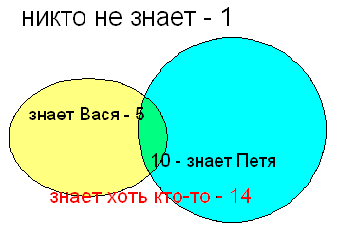
\includegraphics[width=0.9\columnwidth]{./img/Petr}
\end{minipage}
\end{figure}}

\begin{thm}
В толковом словаре для информатиков можно насчитать всего 10 понятных русских слов, и столько же (т.е. 10) непонятных иностранных слов. Чего в словаре больше: понятных слов или иностранных слов?
\end{thm}
{\setlength{\intextsep}{2pt}
\begin{figure}[H]
\begin{minipage}{0.45\linewidth}
    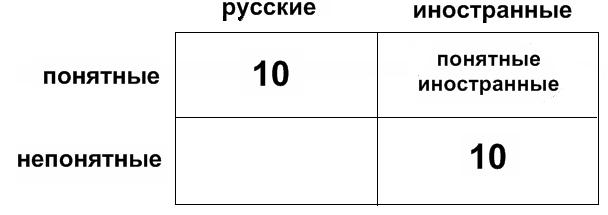
\includegraphics[width=0.95\columnwidth]{./img/shema_slova}
\end{minipage}
\hfill
\begin{minipage}{0.54\linewidth}\setlength{\parindent}{1.5em}
    \begin{prf} Нарисуем условие в виде схемы. Понятных слов в словаре всего на 10 больше, чем понятных иностранных слов (к понятным иностранным прибавляется ещё 10 понятных русских). Но и иностранных слов всего на 10 больше, чем тех же самых понятных иностранных (т.к. к ним прибавляется ещё 10 непонятных иностранных), а значит и тех и других слов в словаре одинаково.
    \par
    \textbf{\textit{Ответ:}} одинаково.
    \end{prf}
\end{minipage}
\end{figure}}

\begin{thm}
Докажите, что для любых множеств $A$, $B$ и $C$ справедливо соотношение:
\par $(A \cup B) \backslash C = (A \backslash C) \cup (B \backslash C)$.
\end{thm}

\begin{prf}
Если мы докажем, что все элементы множества из левой части принадлежат множеству из правой части требуемого равенства и наоборот: все элементы множества из правой части принадлежат множеству из левой части, то утверждение будет доказано.

1)~Пусть элемент $x \in (A \cup B) \backslash C$. Это значит, что $x$ принадлежит объединению множеств $A$ и $B$ и не принадлежит множеству $C$. Если $x \in (A \cup B)$, то это значит, что он обязательно принадлежит или $A$, или $B$. Поэтому, если $x \in A$, то, т.к. он не принадлежит $C$, то он принадлежит $(A \backslash C)$. Аналогично, если $x \in B$, то он принадлежит $(B \backslash C)$. Т.е. в любом случае $х \in (A \backslash C) \cup (B \backslash C)$.

2)~Пусть теперь $х \in (A \backslash C) \cup (B \backslash C)$. Если $х \in (A \backslash C)$, то в частности он принадлежит $A$, если же $х \in (В \backslash C)$, то он принадлежит $B$. Следовательно, в любом случае $x \in (A \cup B)$. Но $x$ не принадлежит $C$, т.к. ни множество ($A \backslash C)$, ни множество $(B \backslash C)$ не имеют с $C$ общих элементов. Таким образом, $х \in (A \cup B) \backslash C$. 
\end{prf}

\begin{thm} 
Известно, что доля блондинов среди голубоглазых больше, чем доля блондинов среди всех людей. Что больше: доля голубоглазых среди блондинов или доля голубоглазых среди всех людей?
\end{thm}
\par
\textbf{\underline{Ответ:}} доля голубоглазых среди блондинов больше.

\begin{prf}
Введем обозначения: \textit{Б} – все блондины, \textit{Г} – все голубоглазые, \textit{бг} – голубоглазые блондины и \textit{Л} – все люди. Тогда запишем, что дано в условии: $\frac{\textit{бг}}{\textit{Г}} > \frac{\textit{Б}}{\textit{Л}}$ (*). Требуется сравнить $\frac{\textit{бг}}{\textit{Б}} и \frac{\textit{Г}}{\textit{Л}}$. \\
Заметим, что произведение чисел \textit{Б} и \textit{Г} положительно, поскольку это количество людей, каждое из которых отлично от нуля. Поэтому, помножив обе части и неравенства (*) на дробь $\frac{\textit{Г}}{\textit{Б}}$, мы не изменим его знака. Имеем:
$\frac{\textit{бг}}{\textit{Г}} \times \frac{\textit{Г}}{\textit{Б}} > \frac{\textit{Б}}{\textit{Л}} \times \frac{\textit{Г}}{\textit{Б}} \Leftrightarrow \frac{\textit{бг}}{\textit{Б}} > \frac{\textit{Г}}{\textit{Л}}$, т.е. доля голубоглазых среди блондинов больше.
\end{prf}

\begin{thm}
В стране Чудаков живут только философы и математики, причём каждый двенадцатый математик - философ, а каждый тринадцатый философ – математик. Какой процент составляют философы?
\end{thm}
\par
\textbf{\underline{Ответ:}} $54\frac{1}{6}\%$.

\begin{figure}[H]
\begin{minipage}{0.7\linewidth}\setlength{\parindent}{1.5em}
    \begin{prf} 
    Пусть количество людей, являющихся одновременно и философами, и математиками, равно $x$ (см. рис.). Тогда математиков $12x$, а философов – $13x$. Поскольку математики-философы учитываются в обоих множествах, то общее количество людей в стране Чудаков равно $12x + 13x - x = 24x$. Теперь легко сосчитать процент:
    \par
    Процент философов = $\frac{\textit{количество философов}}{\textit{количество всех жителей}} \times 100\% = \frac{13x}{24x} \times 100\% = 54\frac{1}{6}\%$.
    \end{prf}
\end{minipage}
\hfill
\begin{minipage}{0.25\linewidth}%\setlength{\parindent}{1.5em}
    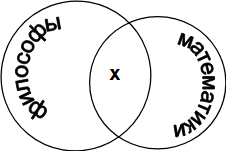
\includegraphics[width=0.9\columnwidth]{img/filosof.png}
\end{minipage}
\end{figure}

\section{Ответы к упражнениям}

\textbf{\ref{5.0 u1}.} а)~$\{1; 2; 3; 4; 6; 12\}$; б) серединный перпендикуляр; в) точка – пересечение серединных перпендикуляров треугольника; г) $\varnothing$ - пустое множество; д) две перпендикулярные прямые, являющиеся биссектрисами углов образованных этими прямыми; е) $\{\textit{С; П; Е; Ц; М; А; Т; И; К; А}\}$. 
\textbf{\ref{5.0 u3}.} Например так: $A \cap B = A~\backslash~(A~\backslash~B)$
\textbf{\ref{5.0 u3}.} Например так: $A \cap B = A~\backslash~(A~\backslash~B)$
\textbf{\ref{5.0 u4}.} 

\begin{minipage}[h]{0.9\linewidth}
\centering
    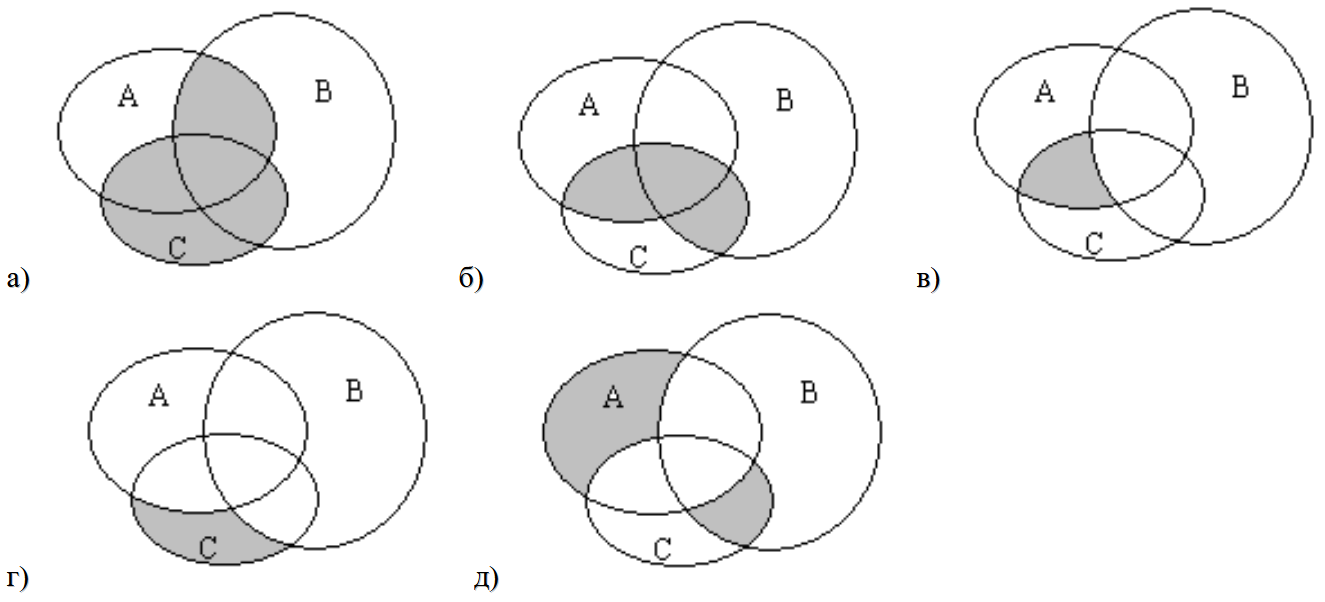
\includegraphics[scale=0.4]{./img/50_otveti}
\end{minipage}
\par
\textbf{\ref{5.0 u5}.} Частичные ответы: 
\par
$A \cap B = \{3; 4; 5; 8\};$ $B \cap C \cap D = \{8; 10\};$ $A \cap B \cap C \cap D = \{8\};$ $A \cup = \{1; 2; 3; 4; 5; 6; 7; 8; 9; 10; 11; 12\} = A \cup B \cup C \cup D$